\documentclass[11pt, a4paper]{book}
\usepackage{MathLetter}
\usepackage{tkz-graph}
\usepackage{tkz-berge}

\usepackage{algorithm}
\usepackage{algorithmic}

\fontsettingfalse%true
\mergedcounterfalse%true

\setcounter{issue}{0}
\setcounter{page}{1}

\title{매트로이드와 그리디 알고리즘}
\author{한국과학기술원 새내기과정학부 이종서}
\date{\today}

\renewcommand{\thealgorithm}{}
\newcommand{\I}{\mathcal{I}}
\newcommand{\A}{\mathcal{A}}

\begin{document}
    \maketitle
    \section{매트로이드란 무엇인가}
    \begin{MLDef}
        어떤 (유한) 집합 $S \neq \emptyset$와 $\I \subseteq 2^S$가 있을 때, $M = (S, \I)$가 \newterm{매트로이드}[matroid]임은 다음의 세 조건을 만족함을 의미합니다.
        \begin{enumerate}
            \item[(M1)] $\emptyset \in \I$이다.
            \item[(M2)] $X \in \I$이고 $Y \subseteq X$이면 $Y \in \I$이다. (유전성\,{\small hereditary})
            \item[(M3)] $X, Y \in \I$가 $|X| < |Y|$를 만족하면, 어떤 $e \in Y - X$가 존재하여, $X \cup \{ e \} \in I$이다. (교환성\,{\small exchange property})
        \end{enumerate}
    \end{MLDef}
    
    실제 매트로이드가 되는 예시를 몇 가지 살펴봅시다. 다음과 같은 그래프 $G$를 생각합시다.
    \begin{center}
    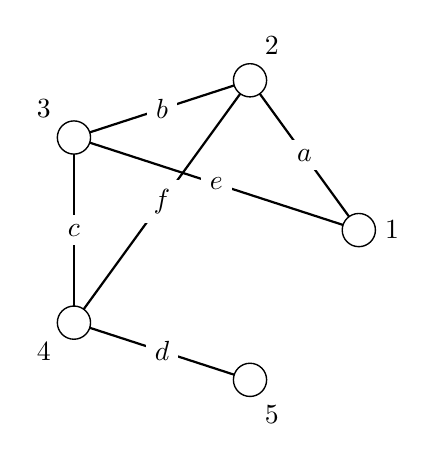
\begin{tikzpicture}
        \GraphInit[vstyle=Welsh]
        \SetGraphUnit{2}
        \Vertices{circle}{1, 2, 3, 4, 5}
        \Edges[label=$a$](1, 2)
        \Edges[label=$b$](2, 3)
        \Edges[label=$c$](3, 4)
        \Edges[label=$d$](4, 5)
        \Edges[label=$e$](1, 3)
        \Edges[label=$f$](2, 4)
    \end{tikzpicture}
    \end{center}
    
    이 그래프 $G$에 대해 $S_G$와 $\I_G$를 다음과 같이 정의합시다.
    \begin{itemize}
        \item $S_G  = \{a, b, c, d, e, f \}$
        \item $\I_G = \{A \subseteq S_G : A\text{에 속하는 간선들이 사이클을 이루지 않음}\}$
    \end{itemize}
    즉, 각 $\I_G$의 원소는 사이클을 이루지 않게 몇 개의 간선을 잘 택해 모아둔 것이 됩니다. 예를 들어, $\{a, b, c, d\}$와 $\{a, d, e\}$는 사이클을 이루지 않으므로 $\I_G$에 속하지만, $\{a, b, e\}$와 $\{a, b, c, f\}$는 사이클을 이루므로 $\I_G$에 속하지 않습니다.
    
    $M_G = (S_G, \I_G)$가 실제로 매트로이드가 되는지 살펴봅시다. 먼저, 공집합이 $\I_G$에 속함은 명백하므로 (M1)을 만족합니다. 또한, 사이클을 이루지 않는 간선들 중 일부를 택하면 여전히 사이클을 이루지 않으므로 유전성(M2)을 만족함 또한 명백합니다. 교환성(M3)을 만족함을 보이는 것은 살짝 까다로운데, 경우를 잘 나누어 따져주면 됩니다. 연습문제로 남겨둡니다.
    
    이 예를 확장하여 다음과 같이 \newterm{그래프 매트로이드}[graphic matroid]를 정의할 수 있습니다.
    
    \begin{MLDef}
        그래프 $G = (V, E)$에 대해 그래프 매트로이드 $M_G = (S_G, \I_G)$는 다음과 같이 정의됩니다.
        \begin{itemize}
            \item $S_G = E$
            \item $\I_G = \{A \subseteq S_G : A\text{에 속하는 간선들이 사이클을 이루지 않음}\}$
        \end{itemize}
    \end{MLDef}
    
    앞서 살펴본 `예시 그래프'에서 $M_G$가 매트로이드임은 쉽게 확인할 수 있었습니다. 일반적인 그래프에 대해서도 (M1)과 (M2)가 성립함은 매우 명백합니다. 하지만, (M3)가 성립함은 그리 자명해보이지는 않습니다. 그래프 매트로이드가 \textbf{실제로} 매트로이드가 되는지 확인해봅시다.
    
    \begin{MLThm}
        임의의 그래프 $G = (V, E)$에 대해 그래프 매트로이드는 실제로 매트로이드입니다.
    \end{MLThm}
    
    \begin{MLPrf}
        (M3)를 만족함만 보이면 충분하므로, (M3)를 만족함을 보입시다.
        
        임의의 $A, B \in \I_G$이고 $|A| < |B|$인 $A$와 $B$를 잡읍시다. 그러면, $A$에는 $|V|-|A|$개의 컴포넌트가 있으며, $B$에는 $|V|-|B|$개의 컴포넌트가 있습니다. $|V|-|A| > |V|-|B|$이므로, 두 정점 $x, y$가 존재해 $A$에서는 다른 컴포넌트에 속하지만 $B$에서는 같은 컴포넌트에 속합니다.
        
        위와 같은 $x, y$를 택한 후, $B$ 상에서 $x$에서 $y$로 가는 경로를 생각해주면, 어떤 $u$와 $v$가 존재해 $x$에서 $y$로 가는 경로상에서 $u$와 $v$를 차례로 지나지만, $A$에서는 다른 컴포넌트에 속하게 됩니다. 즉, $u$와 $v$를 잇는 간선을 $e \in B - A$라 하면, $A \cup \{e\}$ 또한 여전히 사이클을 이루지 않아 $A \cup \{e\} \in \I_G$가 됩니다.
    \end{MLPrf}
    
    위의 증명에 이어서 매트로이드가 되기 위한 여러 조건 중 (M3) 조건에 대해 계속 살펴봅시다. 우선, (M3) 조건의 `원소를 추가하는 행위'에 관련하여 새로운 용어를 정의합시다.
    
    \begin{MLDef}
        매트로이드 $M = (S, \I)$와 $\I$의 원소 $A$가 주어졌을 때, 다음 용어를 정의합니다.
        \begin{itemize}
            \item $x \in S - A$가 $A$의 \newterm{확장}[extension]임은 $A \cup \{x\} \in \I$임을 의미합니다.
            \item $A$가 $M$의 \newterm{극대}[maximal] 원소임은 어떠한 $B \in \I$도 $A$를 부분집합으로 포함하지 않음을 의미합니다.
            \begin{itemize}
                \item 다른 말로, $A$의 확장이 없음을 의미합니다.
            \end{itemize}
            \item $\I^\top$을 $\I^\top = \{ A \in \I : A\text{는 극대원소}$로 정의합니다.
        \end{itemize}
    \end{MLDef}
    
    그래프 $G$가 있을 때, $M_G = (S_G, \I_G)$에서 확장과 극대원소에 대해 살펴봅시다. $A \in \I_G$의 확장은 $A$의 서로 다른 두 컴포넌트를 잇는 간선이 될 것입니다. $A \in I_G$가 극대 원소임은 $A$가 $G$의 각각의 컴포넌트에서 트리를 이룸을 의미합니다. 이로부터 $M_G$의 모든 극대 원소의 크기는 $|V| - (G\text{의 컴포넌트의 갯수})$로 일정함을 알 수 있습니다.
    
    사실, 모든 극대 원소의 크기가 일정하다는 성질은 그래프 매트로이드를 넘어서서 모든 매트로이드에 대해 성립합니다. 이를 매트로이드의 교환성(M3) 조건을 통해 증명해봅시다.
    
    \begin{MLPrp}
        매트로이드 $M = (S, \I)$에 대해 $\I^\top$의 모든 원소의 크기는 같다.
    \end{MLPrp}
    
    \begin{MLPrf}
        귀류법을 통해 증명해봅시다. $A, B \in \I^\top$이 $|A| < |B|$를 만족한다고 가정합시다. 그러면, 교환성(M3)에 의해 $e \in B-A$가 존재해 $A \cup \{e\} \in \I$가 됩니다. $A$의 확장이 존재하므로 $A$는 극대원소가 아니며, 이는 모순입니다.
        
        따라서, $A, B \in \I^\top$이면 $|A| = |B|$입니다.
    \end{MLPrf}
    
    \section{가중치 있는 매트로이드}
    
    우리가 그래프에 대해 생각할 때 종종 간선에 가중치를 부여하여 생각하곤 합니다. 비슷하게, 매트로이드 $M = (S, \I)$가 있을 때, $S$의 원소들에 가중치를 부여하는 상황을 생각해봅시다.
    
    \begin{MLDef}
        가중치 있는 매트로이드와 관련 개념을 다음과 같이 정의합니다.
        \begin{itemize}
            \item $M = (S, \I, w)$가 가중치 있는 매트로이드임은 $(S, \I)$가 매트로이드이고, $w$가 $w : S \to \mathbb{R}_{\ge 0}$임으로 정의됩니다.
            \item $S$의 부분집합 $A$에 대해 $w(A) = \sum_{e \in A} w(e)$로 정의합니다.
            \item $\I^{\star}$를 $\I^{\star} = \{ A \in \I : w(A)\text{가 최대} \}$로 정의합니다. 즉, $\I^{\star}$는 가중치의 합이 가장 큰 $\I$의 원소들의 집합입니다.
            \item $w(\I^{\star})$를 $A \in I^{\star}$의 $w(A)$로 정의합니다. 다시 말해, $w(\I^{\star}) = \max \{ w(A) : A \in \I \}$ 입니다.
        \end{itemize}
    \end{MLDef}
    
    $S$의 원소들을 가중치 순으로 정렬하여 생각합시다.즉, $S = \{x_1, \cdots, x_n \}$이라 할 때, $w(x_1) \ge w(x_2) \ge \cdots \ge w(x_n)$이라 합시다. 다음의 보조정리가 성립합니다.
    
    \begin{MLLem}
        $x_i$가 $\{x_i\} \in \I$인 최소의 $1 \le i \le n$이라 합시다. 즉, $j < i$에 대해 $\{x_j\} \not\in \I$이고, $\{x_i\} \in \I$입니다. 이 때, 어떤 $A \in \I^\star$가 존재해 $A$는 $x_i$를 원소로 가집니다.
    \end{MLLem}
    
    \begin{algorithm}
        \caption{$A$를 구성하는 알고리즘}
        \begin{algorithmic}
            \STATE $A := \{x_i\}$
            \WHILE{$|A| < |B|$}
                \STATE  $A \cup \{x^\prime\} \in \I$인 $x^\prime \in B - A$를 하나 택한다.\\// (M3)에 의해 이런 $x^\prime$의 존재성이 보장됨
                \STATE $A := A \cup \{ x^\prime\}$
            \ENDWHILE
        \end{algorithmic}
    \end{algorithm}
    \begin{MLPrf}
        초기에 $A = \{x_i\}$라 하고, 임의의 $B \in \I^\star$를 택합시다. 만약, $x_i \in B$이면 증명이 종료됩니다. 아니라고 가정하고, 위와 같은 방법을 통해 $A$를 귀납적으로 구성합시다.
        
        이제, 어떤 $x_j \in B$에 대해 $A = \{x_i\} \cup B - \{x_j\}$가 됩니다. $x_i$의 정의와 (M2)에 의해, $j > i$입니다. 따라서, $w(x_i) \ge w(x_j)$가 되고 다음이 성립하여 증명이 종료됩니다.
        $$ w(\I^\star) \ge w(A) = w(B) - w(x_j) + w(x_i) \ge w(B) = w(\I^\star) $$
    \end{MLPrf}
    
    \begin{MLLem}
        $\{x\} \not\in \I^\star \implies \forall A \in \I, \{x\} \not\in \I$
    \end{MLLem}
    
    위의 보조정리는 (M2)에 의해 자명하게 성립합니다. 이 보조정리에 의해 $\{x\} \not\in \I$이면, $x$를 포함하는 $\I^\star$의 원소가 없음이 명백합니다.
    
    \section{매트로이드의 축소}
    
    매트로이드에서 특정 원소를 없애서 새로운 매트로이드를 얻는 것을 생각해봅시다.
    
    \begin{MLDef}
        가중치 있는 매트로이드 $M = (S, \I, w)$와 $x \in S$가 주어졌을 때, M을 $x$에 의해 \newterm{축소}[contraction] 하여 얻어지는 매트로이드 $M_x = (S_x, \I_x, w_x)$는 다음과 같이 정의됩니다. 단, $S_x \neq \emptyset$이어야 합니다.
        \begin{itemize}
            \item $S_x = \{ y \in S - \{x\} : \{x, y\} \in \I \}$
            \item $\I_x = \{ B \subseteq S - \{x\} : B \cup \{x\} \in \I \}$
            \item $w_x = w|_{S_x}$ (정의역의 축소)
        \end{itemize}
    \end{MLDef}
    
    \begin{MLPrp}
        실제로 매트로이드의 축소 또한 매트로이드가 된다.
    \end{MLPrp}
    
    이 증명의 경우 그리 어렵지 않으므로, 연습문제로 남겨두겠습니다.
    
    매트로이드는 \newterm{최적 부분 구조 성질}[Optimal Substructure Property]을 만족합니다. 이는 다음과 같이 나타낼 수 있습니다.
    
    \begin{MLLem}
        매트로이드 $M = (S, \I, w)$이 주어졌다고 합시다. 어떤 $x \in S$가 다음을 만족한다고 합시다:
        \begin{itemize}
            \item[(조건)] $x$를 포함하는 $\I^\star$의 원소가 존재한다.
        \end{itemize}
        이 때, 임의의 $B \in \I_x^\star$에 대해 $B \cup \{x\} \in \I^\star$이다.
    \end{MLLem}
    
    \begin{MLPrf}
        임의의 (조건)을 만족하는 $x$를 잡읍시다. 그리고, $\A_x$를 $\A_x = \{ A \in \I^\star : x \in A \}$로 정의합시다.
        
        그러면, $A \in \A_x$이면, $A - \{x\} \in \I_x$이고, $w(A) - w(x) = w(A - \{x\}) \le w(\I_x^\star)$가 되므로, $w(\I^\star) \le w(\I_x^\star) + w(x)$가 됩니다. $\cdots(\star)$
        
        $B \in \I_x^\star$이라 합시다. 우리는 $B \cup \{x\} \in \I^\star$임을 보일 것입니다. $w(B) + w(x) = w(B\cup\{x\}) \le w(I^\star)$가 되는데, $(\star)$에 의해, $w(I_x^\star) + w(x) = w(\I^\star)$가 됩니다. 따라서, $w(B \cup \{x\}) = w(I^\star)$가 되고, $B \cup \{x\} \in \I^\star$가 되어 증명이 종료됩니다.
    \end{MLPrf}
    
    \section{매트로이드의 그리디 알고리즘}
    
    다음과 같은 알고리즘을 생각합시다.
    
    \begin{algorithm}
        \caption{매트로이드의 그리디 알고리즘}
        Greedy ($M = (S, I, w)$)
        \begin{algorithmic}
            \STATE $A := \emptyset$
            \STATE $S = \{x_1, x_2, \cdots, x_n\}$이 $w(x_1) \ge w(x_2) \ge \cdots \ge w(x_n)$을 만족하게 정렬한다.
            \FOR{$i:=1$ to $n$}
                \IF{$A \cup \{x_i\} \in \I$}
                    \STATE $A := A \cup \{x_i\}$
                \ENDIF
            \ENDFOR
            \STATE return $A$ // $A \in \I^\star$
        \end{algorithmic}
    \end{algorithm}
    
    \begin{MLThm}
        위의 알고리즘은 $\I^\star$의 원소 중 하나를 반환합니다.
    \end{MLThm}
    
    위 정리가 성립함은 보조정리 1,2, 그리고 보조정리 3에 의해 명백합니다. 덧붙여, 이 알고리즘의 수행시간에 관해 다음의 사실이 성립합니다.
    
    \begin{MLPrp}
        If 문의 수행시간이 $\mathcal{O}(f(n))$이라 할 때, 매트로이드의 그리디 알고리즘의 시간복잡도는 $\mathcal{O}(n \log n + n f(n))$이다.
    \end{MLPrp}
    
    \section{매트로이드와 그리디 알고리즘의 활용}
    
    크루스칼의 최소/최대 가중치의 신장트리를 구하는 알고리즘은 널리 알려져 있으며, 다음과 같습니다. (단, 입력으로 주어지는 그래프가 연결 그래프라 가정합시다.)
    
    \begin{algorithm}
        SpanningTree ($G = (V, E, w)$)
        \begin{algorithmic}
            \STATE $T := \emptyset$
            \STATE $E = \{e_1, e_2, \cdots, e_n\}$을 $w(e_1) \ge w(e_2) \ge \cdots \ge w(e_n)$을 만족하게 정렬한다. // 최소 스패닝 트리를 구하는 경우에는 $w(e_1) \le w(e_2) \le \cdots \le w(e_n)$이게 정렬한다.
            \FOR{$i:=1$ to $n$}
                \IF{$T \cup \{e_i\}$가 사이클을 포함하지 않는다}
                    \STATE $T := T \cup \{e_i\}$
                \ENDIF
            \ENDFOR
            \STATE return $T$
        \end{algorithmic}
    \end{algorithm}
    
    이 알고리즘 또한 앞서 살펴본 매트로이드의 그리디 알고리즘으로 부터 자연스레 유도될 수 있습니다. (가중치 있는 그래프 매트로이드를 생각해보세요!)
    
    그러면, 과연 모든 \emph{그리디 알고리즘}을 적용할 수 있는 문제들을 매트로이드로 모델링 할 수 있을까요? 놀랍게도, 그렇습니다!
    
    \begin{MLThm}
        유한 집합 $E$가 주어졌다고 합시다. $\I \in 2^E$가 (M1), (M2)와 다음의 조건을 만족한다고 합시다.
        \begin{itemize}
            \item[(G)] 임의의 가중치 함수 $w : E \to \mathbb{R}_{\ge0}$에 대해 그리디 알고리즘이 올바르게 작동한다.
        \end{itemize}
        이 때, $M = (E, \I)$는 매트로이드가 됩니다.
    \end{MLThm}
    
    \begin{MLPrf}
        (M3)를 만족함만 보이면 충분합니다. $X, Y \in \I$이고, $|X| < |Y|$인 $X, Y$가 주어졌다고 합시다. 귀류법으로 임의의 $e \in Y-X$에 대해 $X \cup \{e\} \not \in \I$라고 합시다. (그러면, 명백하게 $X-Y \neq \emptyset$이 됩니다.)
        
        이제, 작은 양수 $0 < \epsilon < \frac{|Y|-|X|}{|X-Y|}$에 대해 가중치 함수 $w$를
        $$ w(x) = \begin{cases}
            1 + \epsilon & \text{if } x \in X \\
            1 & \text{if } x \in Y - X \\
            0 & \text{otherwise}
            \end{cases} $$
        로 하여 정의합시다. 그러면 그리디 알고리즘을 통해 만들어진 집합을 $X'$라 하면, $X'$는 $X$를 부분집합으로 포함합니다. 따라서, $G$에 의해 $|Y| + \epsilon |X \cap Y| = w(Y) \le w(X') = (1+\epsilon) |X|$가 되는데, 이 식을 정리하면, $\epsilon |X - Y| \ge |Y|-|X|$가 되어 모순이 발생합니다.
        
        따라서, 적절한 $e \in Y - X$에 대해 $X \cup \{e\} \in \I$가 됩니다.
    \end{MLPrf}
    
    \section{결론}
    
    우리는 그리디 알고리즘이 작동하는 거의 모든 문제는 매트로이드로 모델링 할 수 있음을 확인했습니다. 만약, 어떤 문제에 대해 그리디 알고리즘이 작동한다고 생각되면, 그리디 알고리즘이 \emph{정확함}을 보이기 위해 복잡한 증명을 하는 대신 해당 문제가 매트로이드로 모델링 됨을 보이면 될 것입니다.
\end{document}
